\chapter{TensorFlow}
\label{cha:TensorFlow}

TensorFlow repräsentiert eine Bibliothek für Machine Intelligence und entstand in der Google Brain Abteilung.
Das Projekt wird als Open Source Projekt weiterentwickelt, wobei das Projekt von Google weiterhin gepflegt wird. 
Das Offenlegen des Projekts führt dazu, dass auch Personen außerhalb von Google die Möglichkeit bekommen die Bibliothek zu verwenden, sowie auch etwas einflechten können. \newline

\noindent
Das Hauptkonzept hinter TensorFlow sind sogenannte Tensoren, welche einen Graphen durchlaufen. 
%Diese Tensoren werden während ihrem durch lauf verändert und wieder neu zusammengesetzt. 
Der Graph selbst stellt damit einen Datenflussgraphen dar, welcher Knoten beinhaltet. 
Diese Knoten bilden numerische Operationen ab.
Der Informationsaustausch zwischen den Knoten erfolgt mit multidimensionalen Arrays, den Tensoren.
TensorFlow bietet wie andere Bibliotheken die Möglichkeit, die Berechnungen auf eine Grafikkarte auszulagern.
Zusätzlich sind weitere Routinen eingebaut, damit das Trainieren über mehrere Grafikkarten, sowie auf weitere Computer verteilt werden kann. \newline

\noindent
TensorFlow steht für mehrere Programmiersprachen zur Verfügung, welche offiziell unterstützt werden, wobei noch weitere durch die Open Source Gemeinschaft unterstützt werden.
Den Hauptbereich stellt die Python API dar, welche die vollständigste Implementierung enthält. 
Der Kern von TensorFlow ist mit C++ und Python implementiert und wurde sehr stark optimiert, um eine sehr gute Performanz zu erzielen.
Die Python API wird im Umfeld von TensorFlow dazu verwendet, einen Graphen zu erstellen, zu trainieren und zu testen. 
Durch die Verwendung von Python besteht die Möglichkeit, sehr schnell Änderungen am Graphen für die Ergebnisdarstellung durchführen zu können, ohne die ganze Applikationsstrukturen übersetzen zu müssen. 
Dieser Graph wird nach seiner Trainingsphase exportiert und beinhaltet alle Knoten sowie die dazugehörigen Gewichtungen. 
Die C++ API sowie die Java API und GO API zielen auf eine sehr effiziente Ausführung ab.
Durch die Verwendung des trainierten Graphen kann dieser auch auf mobilen Plattformen eingesetzt werden.

\subsection{Graphs/Dataflowgraph}

\begin{lstlisting}[caption={TensorFlow Codefragment zur Definition eines Teils des Graphen},label=fig:SimpleFragmentGraphDefinition,captionpos=b,language=Python]
import tensorflow as tf

b = tf.Variable(tf.zeros([100])) 
	# 100-d Vektor, initialisiert mit 0
W = tf.Variable(tf.random_uniform([784,100],-1,1)) 
	# 784x100 Matrix w/rnd vals
x = tf.placeholder(name="x") 
	# Platzhalter für Eingangsdaten
relu = tf.nn.relu(tf.matmul(W, x) + b) 
	# Relu(Wx+b) Aktivierungsfunktion mit impliziter Addition
C = [...] 
	# Kostenfunktion und noch weitere Knoten
s = tf.Session()
for step in xrange(0, 10):
	input = ...construct 100-D input array ... 
		# Erstellen eines 100-d Vektor mit den Eingangsdaten
	result = s.run(C, feed_dict={x: input}) 
		# Graphen mit den Eingangsdaten ausführen
	print step, result 
		# Ausgabe des Berechneten Resultats
\end{lstlisting}
\begin{figure}
	\centering

\begin{tikzpicture}

	\node[neuron] (x) {x};
	\node[neuron,below=of x] (w) {W};
	
	\node[group,fit={(x) (w)}] (gr1) {};
	
	\node[neuron,right=of x] (MatMul) {MatMul};
	\node[io,below=of MatMul] (b) {b};
	
	\node[group,fit={(x) (MatMul)},right=of x] (gr2) {};
	
	\node[neuron,right=of MatMul] (Add) {Add};
	
	\node[neuron,right=of Add] (ReLU) {ReLU};
	
	\node[neuron,right=of ReLU] (more) {...};
	
	\node[neuron,right=of more] (C) {C};
	
	\draw[conn] (x) -- (MatMul);
	\draw[conn] (w) -- (MatMul);

	\draw[conn] (MatMul) -- (Add);
	\draw[conn] (b) -- (Add);
	
	\draw[conn] (Add) -- (ReLU);
	\draw[conn] (ReLU) -- (more);

	\draw[conn] (more) -- (C);

\end{tikzpicture}

	\caption{Der resultierenden Teilgraph aus dem Codefragment \ref{fig:SimpleFragmentGraphDefinition} nach dem Beispiel in \cite{wp2015tensorflow}}
	\label{fig:SimpleFragmentGraphPic}
\end{figure}
Ein TensorFlow Graph kann wie im Codefragment \ref{fig:SimpleFragmentGraphDefinition} ersichtlich, beschrieben werden und wie in Abbildung \ref{fig:SimpleFragmentGraphPic} grafisch dargestellt werden.
Dieser wurde zum Beispiel mit der Python API erstellt.
Die Knoten und Verbindungen ergeben einen Datenfluss, dieser beinhaltet alle erforderlichen Komponenten, auch für das Persistieren und Aktualisieren der Daten.
Dies sind Erweiterungen für den Hauptgraphen und beinhalten auch Logik für Schleifenverwaltungen.
Ein Knoten in einem Graphen besitzt $0$ bis $n$ Ein- und Ausgänge und eine Kernfunktion. 
Zum Datenhauptfluss mit den Tensoren gibt es zusätzlich spezielle Verbindungen, welche \glqq control dependencies\grqq genannt werden. 
Anhand dieser Verbindungen werden keine Daten im Sinne der Tensoren übertragen, sondern werden herangezogen um Abhängigkeiten zu definieren, wie zum Beispiel eine Ausführung in einem anderen Knoten vor einem anderen zu definieren.
Ein Quellknoten muss die Ausführung abgeschlossen haben, bevor der darauf Wartende mit der Ausführung beginnen kann \cite{wp2015tensorflow}. \\ 

\subsection{Datenfluss Programmierung}

In traditionellen Programmierparadigmen, wie dem Sequenziellen, Prozeduralen oder Imperativen, werden eine Reihe von Operationen definiert welche in einer speziellen Reihenfolge abgearbeitet werden sollen, wie von Neumann beschrieben. 
TensorFlow wird nicht im traditionellen verwendet sonder im Sinne eines Datenflusses. 
Hierbei werden die Bewegungen von Daten in einem Modell beschrieben. 
In diesem Modell existieren Operationen mit explizit definierten Ein- und Ausgängen, wobei die Aktion in der Operation für das Modell verborgen bleibt wie eine \glqq black box\grqq. 
Eine Operation wird ausgeführt sobald alle Eingänge vorhanden und valide sind. 
Dies Art der Programmierung bietet von sich aus die Möglichkeit der parallelen Ausführung, sowie ein Einfaches verteilen der Berechnungen auf ein dezentrales System. 

\subsection{Operation}

Die Operation stellt in jedem Knoten den Kern dar, wie zum Beispiel eine Matrix Multiplikation oder eine Addition.
In TensorFlow selbst gibt es einen Unterschied zwischen Operation und Kernel.
Operationen besitzen Attribute, welche spätestens zum Zeitpunkt der Grapherstellung bekannt sein müssen. 
Ein solches Attribut wäre zum Beispiel, um einer Operation polymorphismus zu ermöglichen.  
Der Kernel hingegen ist die Implementierung der Operation selbst. 
Dieser kann auf verschiedenen Geräten ausgeführt werden, wie zum Beispiel auf der CPU oder GPU.
Die Operationen und die dazugehörigen Kernels werden über einen Registrierungsmechanismus zur Verfügung gestellt. 
Diese Sammlung an Operationen kann auch erweitert werden \cite{wp2015tensorflow}. 

\subsection{Sessions}

Die Session repräsentiert die Laufzeit eines Graphen. 
Dieser Session wird ein Graphen übergeben, welcher zuvor initialisiert werden muss. 
Ohne die Initialisierung der Knoten und Verbindungen würde die weitere Ausführung nichts produzieren, da alle Werte $0$ sind. 
Sie stellt eine weitere Funktion zur Verfügung genannt \textit{Run}. 
Der Run-Funktion wird eine Liste an Endknoten übergeben, welche berechnet werden sollen und die zu dem initialisierten Graphen gehören. 
Die Platzhalter Tensoren werden mit Daten verknüpft und an den Graphen gereicht. 
In den meisten Fällen wird ein Graph einmal erstellt und mehrfach ausgeführt \cite{wp2015tensorflow}. 

\subsection{Tensor}

In TensorFlow ist ein Tensor ein typisiertes multidimensionales Array. 
Die verwendbaren Typen reichen von Datentypen mit und ohne Vorzeichen, sowie bis hin zu Doubles und Zeichenketten  \cite{wp2015tensorflow}. 

\subsection{Hyperparameter} 

Hyperparameter werden im Umfeld von maschinellem Lernen verwendet, um Variationen an Kombinationen zu testen. 
Dabei werden verschiedenste Parameter getestet, wie unterschiedliche Aktivierungsfunktionen oder Optimierungsalgorithmen, aber auch die Anzahl an Ebenen und Breiten dieser. 
Im Gesamten führt dies meist zu sehr vielen Permutationen, welche ausgetestet werden müssen und somit voll trainiert werden. 
Da die Zeit, die dafür benötigt werden würde, nicht in sinnvoller Relation dazu steht, werden solche Brute-Force Tests nur mehr selten durchgeführt. 
Für diesen Fall existieren eigene Techniken, welche sich nur um das Optimieren der Hyperparameter kümmern \cite{bishop2006pattern}. 

\section{Bibliotheksinhalt}

\subsection{Datentypen}

TensorFlow besitzt eine große Anzahl an Datentypen, welche verwendet werden können. 
Diese reichen von Grunddatentypen wie 'Boolean' und 'String' bis hin zu verschiedenen Integer Datentypen. 
Sie stehen in verschiedenen Wertebereichen zur Verfügung. 
Es gibt Gleitkommazahlen mit unterschiedlichen Genauigkeiten. 16-bit steht für eine halbe Genauigkeit und 64-bit Genauigkeit entspricht einer doppelten Genauigkeit.
Der Grund für diese verschiedenen Anzahlen an Datentypen ist, dass diese zur Optimierung verwendet werden können. 
Ein trainiertes Netzwerk, welches nie in den Wertebereich von 64-bit signierte Integers gekommen ist, wird diesen möglicherweise nie benötigen. 
In einem solchen Fall können die Wertebereiche reduziert werden, zum Beispiel auf 32-bit signierte Integer, somit können die Berechnungen hochperformanter ausgeführt werden \cite{TensorFlow}. 

\subsection{Operationen}

\subsubsection{Konstanten und Zufallswerte}

\paragraph{Konstanten} liegen in TensorFlow vordefiniert zur Verwendung.
Diese stellen initialisierte Tensoren für den ersten Trainingsdurchlauf zur Verfügung.

\begin{itemize}
	\item \textit{tf.zeros} erstellt einen Tensor mit den angegebenen Matrizendimensionen, bestehend aus $0$ und von einem definierten Datentypen. 
	\item \textit{tf.zeros\_like} gibt einen Tensor zurück, welcher dieselben Dimensionen wiedergegeben besitzt.
	Alle Werte in diesem Tensor sind auf $0$ gesetzt.
	In diesem Schritt kann der Datentyp mit angepasst werden, wenn die Dimensionen übernommen werden sollen.
	\item \textit{tf.ones} agiert genau wie der Tensor \textit{tf.zeros}, mit dem Unterschied, dass alles mit $1$ gefüllt wird.
	\item \textit{tf.ones\_like} repräsentiert dasselbe wie \textit{tf.zeros\_like}, jedoch mit dem Wert $1$.
	\item \textit{tf.fill} fügt eine neue Dimension in einen Tensor ein, mit dem gegebenen Skalar, der für die Werte eingesetzt werden soll.
	\item \textit{tf.constant} liefert einen Tensor mit selbst definierbaren Werten. 
	Diese Werte können sowohl eine Liste sein, als auch ein einzelner Wert, welcher beliebig eingefügt werden soll. 
\end{itemize}

\paragraph{Sequenzen} können verwendet werden, um einen Wertebereich in eine bestimmte Anzahl an Werte zu zerteilen und diese als Tensor in das System wieder einfließen zu lassen.

\begin{itemize}
	\item \textit{tf.lin\_space} generiert einen eindimensionalen Tensor vom Datentypen $32$ oder $64$-bit Gleitkommazahl, mit einer bestimmten Folge.
	Diese beginnt mit einem Startwert und endet mit dem Endwert. 
	Die Werte, welche innerhalb dieses Bereiches liegen, werden gleichmäßig verteilt. 
	\item \textit{tf.range} erstellt wie \textit{tf.lin\_space} einen eindimensionalen Tensor mit Skalarwerten. 
	Die Folge beginnt mit einem Startwert und erweitert sich um ein bestimmtes Delta bis zum Endwert, welcher nicht Teil der Folge ist. 
\end{itemize}

\paragraph{Zufallswerte} werden im Bereich von maschinellem Lernen sehr häufig benötigt. 
So wird der Startzustand oft mithilfe von Zufallszahlen hergestellt. 

\begin{itemize}
	\item \textit{tf.random\_normal} liefert einen Tensor mit Zufallswerten anhand einer Normalverteilung (Gaussian). 
	Die Dimension des Ergebnistensors muss spezifiziert werden, der Median, die Standardabweichung sowie der resultierende Datentyp können angegeben werden. 
	\item \textit{tf.truncated\_normal} verhält sich gleich zu \textit{tf.random\_normal} mit dem Unterschied, dass bei Werten die größer als $2$-mal die Standardabweichung sind, diese ignoriert werden und ein neuer Wert ausgewählt wird.
	\item \textit{tf.random\_uniform} generiert einen Tensor, in welchem Werte gleich wahrscheinlich vorkommen.
	Die Werte werden aus dem spezifizierten Wertebereich genommen, wobei diese exklusiv der oberen Grenze entsprechen (siehe Beispiel '$[0, 1)$').
	\item \textit{tf.random\_shuffle} erstellt eigenständig keine neuen Werte, sondern mischt einen Tensor anhand seiner ersten Dimension durch. 
	\item \textit{tf.random\_crop} liefert einen zufälligen Teil eines Tensors mit derselben Anzahl an Dimensionen jedoch mit der spezifizierten Größe.
\end{itemize} \phantom \newline

\noindent
Einige dieser Funktionen benötigen sogenannte Seed-Werte, welche für die zufällige Verteilung der Startwert benötigt werden. 
Im Falle von TensorFlow beruht dies auf zwei Werten, einer wird für den Graphen spezifiziert, der andere für Operationen selbst. 
Der Wert für den Graphen kann mit \textit{tf.set\_random\_seed} gesetzt werden. 
Für weitere Informationen steht die online Dokumentation zur Verfügung. \footnote{Online Dokumentation: Constants, Sequences, and Random Values  \url{www.tensorflow.org/api_guides/python/constant_op}}

\subsubsection{Variables}

Variablen geben bei jedem Durchlauf einen Tensor ab.
Dieser Wert ändert sich solange nicht, bis ihm ein neuer Wert zugewiesen wird. 

\subsubsection{Transformationen}

\paragraph{Casting} bietet die Möglichkeit wie in anderen Programmiersprachen Typen zu konvertieren. 
Diese Operation muss in den Graphen eingepflegt werden, da keine impliziten Konvertierungen durchgeführt werden. 
Es kann jeder Tensor konvertiert werden, sowie eine Zeichenfolge in eine Zahl. 
Bei diesem Vorgang kann ein Fehler entstehen, welcher in einem \textit{TypeError} resultiert.

\paragraph{Shapes und Shaping} liefern die Gestalt eines Tensors, bieten jedoch auch die Möglichkeit an, diese zu ändern. 
\begin{itemize}
	\item \textit{tf.shape} liefert eine genaue Aufschlüsselung des Tensors mit der Dimension und der Tiefe.
	\item \textit{tf.size} repräsentiert die Anzahl an Elementen in einem Tensor. 
	Diese Anzahl ergibt sich aus den konkreten Werten.
	\item \textit{tf.rank} verhält sich ähnlich zu \textit{tf.size} mit dem Unterschied, dass die Anzahl der Dimensionen gezählt werden.
	\item \textit{tf.reshape} wird verwendet, um Tensoren in eine neue Struktur zu bringen. 
	Dabei steht für das Einebnen der Struktur auf eine Ebene eine Kurzschreibweise zur Verfügung, mit $-1$ als Zieldefinition. 
%	Dabei kann für das Einebnen der Dimensionen eine Kurzschreibweise verwendet werden, mit $-1$ als Zielausführung der Gestalt.
	\item \textit{tf.squeeze} entfernt ganze Dimensionen aus dem gegebenen Tensor. 
	Ohne Achsenangabe werden alle Dimensionen mit der Größe $1$ entfernt oder es werden die spezifizierten Dimensionen herausgenommen.
	\item \textit{tf.expand\_dims} gliedert eine Dimension in einen Tensor wieder ein. 
	Standardmäßig an der Indexstelle $0$, außer es wurde spezifiziert.
\end{itemize}

\paragraph{Slicing und Joining} wird wie in diversen Programmiersprachen auch von TensorFlow unterstützt, im Speziellen mit Tensoren. 
Diese Operationen reichen von einfachen Slicing Operationen über Transponieren bis hin zu dem Verketten von Tensoren. 
Dabei kann definiert werden, anhand welcher Achse der Dimensionen die Operation ausgeführt werden soll.  
%\paragraph{Fake quantization} => zu viel
\phantom \newline

\noindent
Weiter Informationen befinden sich in der online Dokumentation. \footnote{Online Dokumentation: Tensor Transformations \url{www.tensorflow.org/api_guides/python/array_ops}}

\subsubsection{Mathematik} 

\paragraph{Arithmetische Operationen} stellen die mathematischen Grundoperationen dar. 
Diese können teilweise in Kurzschreibweisen verwendet werden, wie zum Beispiel die Addition. 
Sie kann entweder als explizite Operation \textit{tf.add(x, y)} verwendet werden aber auch implizit bei der Addition $+$ von einem Tensor mit einem Bias-Tensor.

\paragraph{Basis Funktionen} ergänzen die arithmetischen Operationen um Standardfunktionen. 
Zu diesen Funktionen zählen die Berechnung der Absolutwerte in einem Tensor sowie eine Exponentialfunktion. 

\paragraph{Matrizen Funktionen} werden am häufigsten benötigt, da Tensoren im Grunde aus Matrizen bestehen und  diese geändert werden können. 
\begin{itemize}
	\item \textit{tf.matmul} führt eine Matrizenmultiplikation aus. 
	Diese Operation findest meist in voll vernetzten Neuronen Verwendung, wenn der übergebene Tensor mit der Gewichtung multipliziert wird. 
	\item \textit{tf.eye} erzeugt eine Identitätsmatrix, in welcher alle Werte entlang der Diagonale $1$ sind und alle anderen den Wert $0$ bekommen. 
\end{itemize}

\noindent
Zu diesen Funktionen existieren noch weitere Ansätze, die zur Lösung von Gleichungen verwendet werden können. 
Diese Gleichungen müssen in Matrizenschreibweise im Tensor abgebildet sein. 

\paragraph{Komplexe Zahlen} können verwendet werden und Operationen mit ihnen in die Graphen eingepflegt werden. 

\paragraph{Reduzierungsoperationen} kommen dann zum Einsatz, wenn der Unterschied zwischen dem erzielten und dem erwarteten Ergebnis festgestellt werden soll. 
\begin{itemize}
	\item \textit{tf.reduce\_sum} berechnet die Summe aller Werte in einem Tensor.
	\item \textit{tf.reduce\_mean} berechnet das arithmetische Mittel eines Tensors. 
	\item \textit{tf.reduce\_max} reduziert einen Tensor auf die maximalen Werte in der letzten Dimension und reduziert dabei den Rang um eins.
\end{itemize}

\noindent
Zu diesen gibt es noch weitere, welche in diversen Fällen benötigt werden, zum Beispiel, wenn Wahrheitswerte reduziert werden sollen. \newline

\noindent
Die Anzahl an mathematischen Funktionen ist sehr viel größer, als die hier Erwähnten. 
Die hier Angeführten repräsentieren lediglich die meist verwendeten Operationen. 
Für weitere Informationen steht die online Dokumentation zur Verfügung. \footnote{Online Dokumentation: Math  \url{www.tensorflow.org/api_guides/python/math_ops}}

\subsubsection{Flusskontrolle}

\paragraph{Flusskontrollen} sind Operationen, die den Ablauf im Graphen beeinflussen. 
Dies können Bedingungen, wie im Sinne von \textit{if (Bedingung)\{...\} else \{...\}} aber auch \textit{switch (Term) \{ case '0': ...; break;\}} Bedingungen sein. 
In beiden Fällen müssen die auszuführenden Verzweigungen als Funktionen vorliegen. 
Zusätzlich gibt es noch eine \textit{While} und eine \textit{For} Schleife. 
Zu beachten ist, dass diese Operationen den Fluss durch den Graphen stark beeinträchtigen können.

\paragraph{Logik Operatoren} können verwendet werden, um Vergleiche zwischen Tensoren durchzuführen. 
Diese werden aber als Logik Operationen ausgeführt und liefern immer Wahrheitswerte, wie eine logische Und-Verknüpfung auf Binärebene.

\paragraph{Vergleichsoperatoren} sind neben den logischen Operatoren weitere Vergleichsoperatoren, welche zur Verfügung stehen. 
Hierzu zählen \textit{tf.equal} sowie die verneinte Variante \textit{tf.less} und \textit{tf.greater} mit jeweils einer gleichen Version. 
Diese Operatoren geben wiederum einen Tensor mit Wahrheitswerten aus.

\paragraph{Debugging Operationen} ermöglichen es in den Graphen Kontrollstrukturen einzubauen, welche auf diverse Bedingungen reagieren.
So kann überprüft werden, ob ein Tensor Werte mit undefinierten Zustand beinhaltet. 
Die Funktion \textit{tf.Print} ermöglicht es Tensoren auszugeben, wenn diese als Funktion im Graphen evaluiert werden. 
Aktuell sind die Möglichkeiten einen Graphen zu debuggen relativ eingeschränkt. 
Grund dafür ist, dass der Graph, in seiner rohen Darstellung schwer zu verstehen ist. \footnote{Online Dokumentation: Control Flow \url{www.tensorflow.org/api_guides/python/control_flow_ops}}

\subsubsection{Images}

\paragraph{Encodieren und Decodieren} von Bilddateien wird in TensorFlow direkt unterstützt.
Dabei können Bilder der Datentypen Gif, Jpeg und PNG gelesen werden, sowie das Erstellen von Bildern in diese Datentypen, ausgenommen Gif.
In allen Fällen wird das Bild als Zeichenkette mit Pfad angegeben. 

\paragraph{Größenänderung} von Bildern ist erforderlich, da im Laufe der Zeit sehr wahrscheinlich größere Bilder verwendet werden, diese aber nicht in das fixe Raster des Netzwerkes passen. 
Für die Größenänderung stehen mehrere Implementierungen mit unterschiedlichen Algorithmen zur Verfügung.

\paragraph{Beschneiden} wird dann benötigt, wenn aus einem Bild ein Teil herausgenommen werden soll. 
Zum Herausnehmen stehen wiederum mehrere Operationen zur Verfügung, welche mit umschließenden Boxen arbeiten oder wie viel Prozent von der Mitte des Bildes aus verwendet werden soll.

\paragraph{Flippen, Rotieren und Transponieren} ermöglicht es, Bilder zu verändern, sodass es für einen Menschen mehr oder weniger noch dieselbe Bedeutung hat, jedoch nicht mehr für einen Computer. 
Für diesen stellt ein rotiertes oder gespiegeltes Bild ein neues Bild dar. 
Diese Technik wird beim Trainieren von Bilderkennungen eingesetzt, um zum Beispiel aus geringen Datenmengen, die zum Trainieren verfügbar sind, mehrere zu generieren. \phantom \newline

\noindent
Zusätzlich gibt es noch die Möglichkeit die Farbkanäle des Bildes zu ändern sowie das Bild nachzujustieren. 
\footnote{Online Dokumentation: Images \url{www.tensorflow.org/api_guides/python/image}}

\subsubsection{Input und Readers}

\paragraph{Platzhalter} werden benötigt, um einen Graphen zu erstellen. 
Ohne Platzhalter können keine Daten in den Graphen von außerhalb geladen werden. 
Diese müssen zur Ausführungszeit durch echte Daten ersetzt werden. 
Dies erfolgt mit Hilfe eines Schlüssen-Wert-Paars in der Run-Methode der Session. 

\paragraph{Readers} ermöglichen es, aus dem Dateisystem Daten direkt zu laden. 
Dabei stehen spezifizierte Reader zur Verfügung, welche Tensoren direkt ausliefern, sowie Zeile für Zeile  oder ganze Dateiinhalte liefern. 

\paragraph{Konvertierungsoperationen} ermöglichen es, Dateien, die mit TensorFlow Readers gelesen wurden weiter zu verarbeiten, so kann zum Beispiel eine CSV Datei decodiert verwendet werden.
\phantom \newline

\noindent
Des Weiteren sind Protokoll Buffer sowie Queues implementiert, die zum Vorverarbeiten von Daten dienen.
\footnote{Online Dokumentation: Input und Readers \url{www.tensorflow.org/api_guides/python/io_ops}}

\subsubsection{Neuronale Netzwerke}

Neuronale Netzwerke sind eine Spezialisierung im Gebiet des maschinellen Lernens. 
TensorFlow bietet eine breite Unterstützung beziehungsweise eine große Implementierungsvielfalt für diesen Typ an. 

\paragraph{Aktivierungsfunktionen} repräsentieren den Ausgang eines Neurons, dabei existieren aus der Vergangenheit einige Ansätze für diesen Bereich eines neuronalen Netzwerkes. 
\begin{itemize}
	\item \textit{tf.sigmoid} ist eine der bekanntesten und ältesten diesen Typs.
	Diese Funktion besitzt im Punkt $0$ einen Aktivierungswert von $0.5$ und hat zwei Beschränkungen. 
	Im negativen Zahlenbereich auf der X-Achse wird der Grenzwert der Funktion mit $0$ definiert und im positiven Zahlenbereich mit dem Grenzwert von maximal $1$. 
	Ein negativer Wert führt somit zu einem geringen Aktivierungswert, welcher sich im Negativen an $0$ annähert sowie im Positiven an $1$.
	In der Abbildung \ref{fig:Sigmoide Aktivierungsfunktion} befindet sich diese Funktion mit ihren Grenzwerten. 
\begin{figure}[ht!]
	\centering
	\resizebox {0.5\linewidth} {5cm} {
	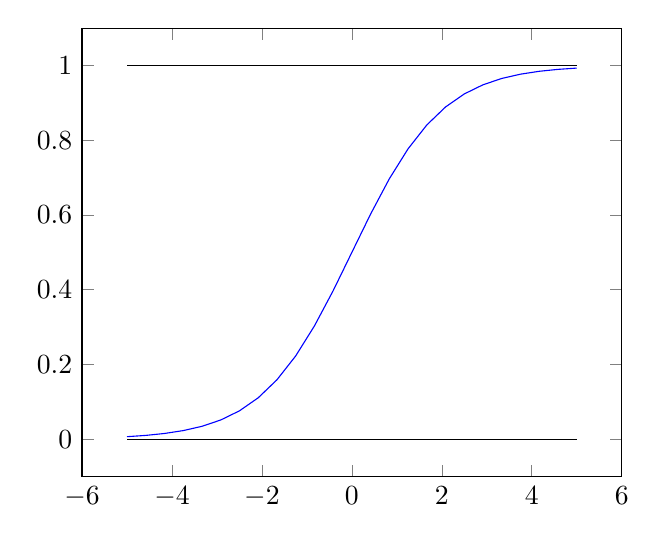
\begin{tikzpicture}
	\begin{axis}

		\addplot[black, no markers] expression {1};
		\addplot[blue, no markers] expression { 1/(1+exp(-x) };
		\addplot[black, no markers] expression {0};

	\end{axis}
	\end{tikzpicture}
	}
	\caption{Sigmoide Aktivierungsfunktion mit den Grenzwerten an den Stellen $1$ und $0$}
	\label{fig:Sigmoide Aktivierungsfunktion}
\end{figure}
	\item \textit{tf.relu} ersetzt mittlerweile immer mehr die sigmoiden Funktionen. 
	Ein Grund dafür ist, dass die Berechnung eines Wertes in einer sigmoiden Funktionen Ressourcen intensiver ist und dass negative Werte meist nicht gewollt sind. 
	Die rektifiziert lineare Funktion ist sehr viel einfacher, da Werte unter $0$ als $0$ weitergegeben werden und Werte darüber linear sind. 
	Somit resultiert ein Eingangswert von $-0.1$ in einer $0$ und ein Wert von $0.5$ in $0.5$.
	Wie in der Abbildung \ref{fig:rektifiziert lineare Aktivierungsfunktion} ersichtlich ist, führt dies bei einem negativen Wert dazu, dass sich eine Multiplikation mit der Gewichtung in der nächsten Ebene ebenfalls in einer $0$ sich repräsentiert und somit in der Addition ignoriert wird.
\begin{figure}[ht!]
	\centering
	\resizebox {!} {5cm} {
	\begin{tikzpicture}
	\begin{axis}

		\addplot[blue, no markers] expression { max(0, x)};

	\end{axis}
	\end{tikzpicture}
	}
	\caption{rektifiziert lineare Aktivierungsfunktion}
	\label{fig:rektifiziert lineare Aktivierungsfunktion}
\end{figure}
	\item \textit{tf.tanh} genannt Hyperbolic Tangent gehört ebenfalls zu den grundlegenden Aktivierungsfunktionen. 
	Der Unterschied zwischen dieser Funktion und der sigmoiden Aktivierungsfunktion ist, dass der untere Grenzwert nicht bei $0$ liegt sondern bei $-1$. 
	In der Abbildung \ref{fig:Hyperbolic Tangents Aktivierungsfunktion} lässt sich erkennen, wo sich der Wendepunkt befindet und liegt im Falle des Hyperbolic Tangent in der Koordinate $x = 0, y = 0$. 
\begin{figure}[ht!]
	\centering
	\resizebox {!} {5cm} { %\linewidth
	\begin{tikzpicture}
	\begin{axis}

		\addplot[black, no markers] expression {1};
		\addplot[blue, no markers] expression { tanh(x)};
		\addplot[black, no markers] expression {-1};

	\end{axis}
	\end{tikzpicture}
	}
	\caption{Hyperbolic Tangents Aktivierungsfunktion mit den Grenzwerten an den Stellen $1$ und $-1$}
	\label{fig:Hyperbolic Tangents Aktivierungsfunktion}
\end{figure}
\end{itemize}
Zu diesen Aktivierungsfunktionen stehen noch einige weitere zur Verfügung, die ausführlich getestet werden sollten. 
Im Grunde kann jede Funktion angewendet werden, doch besitzt jede eine Eigenheit und beeinflusst so den gesamten Graphen. 

\paragraph{Faltung Operationen} werden bei Bilderkennungen unter anderem deshalb verwendet, da eine Operation mit unterschiedlichen Daten in einem Schritt auf mehrere Daten angewendet werden kann. 
%da sie eine Operation auf einen Stapel an Daten gleichzeitig anwenden können. 
Dabei wird ein Fenster über ein Bild geschoben und auf jedem Bild wird im selben Fenster die Operation durchgeführt. 
Diese Operation generalisiert die darunterliegenden Daten so, als ob sie auf etwas reagiert hätten. 
Dies entspricht in etwa dem, als ob ein Auge auf etwas reagiert hätte. 
%https://devblogs.nvidia.com/parallelforall/deep-learning-nutshell-core-concepts/ -> Image by Maurice Peemen.
\begin{itemize}
	\item \textit{tf.nn.conv2d} steht für zweidimensionale Bilder zur Verfügung. 
	\item \textit{tf.nn.conv3d} ermöglicht es mit dreidimensionalen Objekten zu arbeiten.
\end{itemize}
Des Weiteren stehen noch andere spezialisierte Versionen implementiert zur Verfügung.

\paragraph{Bündelung} wird verwendet, um Daten zu vereinfachen, wie zum Beispiel \glqq MaxPool\grqq in Convolutional Netzwerken. 
Eine Faltungsoperation führt dazu, dass aus einem Bild viele mit unterschiedlichen Filtern erzeugt werden.
Eine Bündelung ermöglicht eine Vereinfachung der Daten, wobei die Schlüsselinformationen dennoch erhalten bleiben sollen. 
%die Schlüsselinformationen jedoch bleiben dennoch erhalten. 
%Diese Technik wurde in früheren Zeiten eingesetzt, um Computerressourcen zu sparen, da diese nicht so leistungsfähig gegenüber heute waren. 
TensorFlow bietet mehrere Umsetzungen, so kann sowohl ein Maximalwert aus der Filtermatrix, als auch der Mittelwert übernommen werden. 

\paragraph{Verluste} beschreiben, wie weit ein Ergebnis vom erwarteten Ergebnis entfernt liegt. 
Diese Art der Verlustfeststellung wird bei Regressionsproblemen benötigt, sie haben generell auch die Funktion des Regulierens.
\begin{itemize}
	\item \textit{tf.nn.l2\_loss} berechnet die Hälfte der L2 Norm für den gegebenen Tensor. % deinen Wert, welcher den Inhalt des Tensors repräsentiert. 
	Im Falle dieser Implementierung wird keine Wurzel des Quadrats berechnet, sondern das Ergebnis der Summierung durch $2$ dividiert.
	\item \textit{tf.nn.log\_poisson\_loss} berechnet den logarithmischen Wahrscheinlichkeitsverlust zwischen dem Ergebnis und einem erwarteten Ergebnis. 
	Diese Methode liefert nicht den exakten Verlust, dies stellt in Bezug auf Optimizer (\ref{training}) aber kein Problem dar. 
	Sollte trotzdem ein genauerer Wert bentötigt werden, muss die aufwändige Stirling Approximation \cite{feller1968introduction} aktiviert werden. 
\end{itemize}

\paragraph{Klassifizierungen} repräsentieren einen großen Bereich des maschinellen Lernens. 
TensorFlow besitzt deshalb mehrere Hilfsfunktionen, welche das Arbeiten mit Klassifizierungen erleichtert. 
\begin{itemize}
	\item \textit{tf.nn.softmax} bildet alle Ergebnisse auf einen prozentualen Bereich ab. 
	So ergeben alle möglichen Ausgänge in Summe $100\%$, was so viel bedeutet, dass ein Ergebnis eine gewisse Wahrscheinlichkeit besitzt. 
	\item \textit{tf.nn.softmax\_cross\_entropy\_with\_logits} bietet die Möglichkeit, den Fehlerwert für Diskret-Klassifikationen zu berechnen, wobei jedes Ergebnis genau einer Klasse zugeordnet werden muss. 
	%bietet einem die Möglichkeit auf nicht skalierte Daten ein Ergebnis zu berechnen, welches eine \textit{tf.nn.softmax} Berechnung liefern würde. 
	Diese Funktion kann zum Trainieren verwendet werden, benötigt die unskalierten Werte des Netzwerkes und liefert für jeden Eintrag im Batch einen Fehlerwert. 
	%Zusätzlich wird eine weitere sogenannte 'Cross Entropy' Operation ausgeführt, in welcher das Ergebnis für Optimierungen benötigt wird. 
	%Die gesamte Methode berücksichtigt im gesamten Prozess Spezialfälle, welche schwer manuell zu berücksichtigen sind. 
\end{itemize}
\phantom \newline

\noindent
Zu diesen existieren noch weitere Implementierungen mit weiteren Eigenheiten, welche in diversen Situationen möglicherweise einen Vorteil bieten. 
\phantom \newline
%\paragraph{Wiederkehrend Neuronale Netzwerke} 

\noindent
Des Weiteren gibt es Implementierungen für rekursive neuronale Netzwerke und noch mehr. 
\footnote{Online Dokumentation: Neural Network \url{www.tensorflow.org/api_guides/python/nn}}

\subsubsection{Running Graphs}

\paragraph{Session} stellt eine Hauptklasse des TensorFlow-Systems dar, mit der TensorFlow Engine im Hintergrund.
In ihr werden alle Operationen ausgeführt und alle Tensoren evaluiert. 
Dieser Session wird ein Graphen mitgegeben, in dem der Endpunkt des Graphen angeben wird. 
Zur Ausführungszeit führt die Engine alle Operationen bis zum definierten Endpunkt des Graphen durch und evaluiert die Tensoren in diesem. 
Die Engine führt dabei alles bis zum gegebenen Punkt aus, welcher als Endpunkt übergeben wurde. 
Sollte der Graphen weiterführen, so wird dieser nicht mehr durchlaufen. 
Dies bietet eine eingeschränkte Möglichkeit, um das aufgebaute System zu testen. 
Eine Session wird mit \textit{tf.Session} erstellt und stellt die Funktionalität zum Ausführen, sowie die Möglichkeit, diese zu schließen zur Verfügung. 
Mit \textit{tf.InteractiveSession} wird ebenfalls eine Session erstellt, diese wird aber zugleich als Basissession installiert. 
Dies bietet die Möglichkeit, interaktiv in einer Kommandozeile Operationen auszuführen, ohne die Session expliziert zu übertragen und anzusprechen. 
Die Tensoren und Operatoren bieten in diesem Fall die Option sich und den Graphen auszuführen, indem die Methoden \textit{TensorVariable.eval} sowie \textit{OperationsVariable.run} in diesen aufgerufen werden. 
%Zusätzlich kann eine bestehende Basissession geholt werden sowie auf Fehler reagiert werden. 
\footnote{Online Dokumentation: Running Graphs \url{www.tensorflow.org/api_guides/python/client}}

\subsubsection{Training}
\label{training}

\paragraph{Optimizers} stellen einen weiteren Kernteil des Systems dar. 
TensorFlow stellt eine Menge an implementierten Optimierungsalgorithmen zur Verfügung. 
Diese Operationen trainieren den Graphen mit der gewählten Technik des gewählten Algorithmus. 
Diese Implementierungen versuchen die gegebenen Kosten eines Graphen zu minimieren. 
Bei der Verwendung von \textit{minimize} führt die Operation zwei Schritte in einem aus. 
In diesem wird der Gradient berechnet und dieser wird direkt auf die Variablen adaptiert. 
Diese Schritte können in einzelne zerlegt werden, wenn mit den berechneten Gradienten noch etwas zusätzlich durchgeführt werden soll. 
Die Berechnung wird dabei mit \textit{opt.compute\_gradients} ausgelöst, was eine Liste mit Paaren liefert. 
Diese Liste kann bearbeitet werden, aber auch zu Testzwecken mit protokolliert werden. 
Die Gradienten werden im dritten Schritt mit \textit{opt.apply\_gradients} auf die Variablen angewendet. 
Jeder Optimierungsalgorithmus verfügt über Eigenheiten und spezielle Verhalten, welche bei der Auswahl des Optimierers berücksichtigt werden sollten.

\paragraph{Gradient Computation} umfasst Methoden, die das Verhalten des Graphen und der Optimierung beeinflussen. 
Diese Methoden ermöglichen es, Einfluss auf die Gradientenberechnung sowie auf dessen Evaluierung zu nehmen. 
In diesem Sinne sind diese mit Vorsicht zu verwenden.

\paragraph{Verteilte Ausführung} stellt eine der Stärken von TensorFlow dar, da diese Technologie schon im System integriert ist und somit keine manuelle Verteilung der Aufgaben entwickelt werden muss. 
Dadurch besteht die Option, die Berechnungen auf mehrere Geräte zu verteilen und so die zur Verfügung stehenden Ressourcen besser auszunützen. \\
%Im Grunde wird ein Cluster definiert welcher Computerknoten umfasst. 
%Diesen werden dann Tasks auf Aufgaben zugewiesen, wobei zu den Knoten definiert werden muss was zu tun ist.

\noindent
Einige Komfortmethoden ermöglichen es, einfacher eine Session zu erstellen und alle Variablen zu initialisieren sowie im Anschluss zu trainieren, wobei eine Stoppbedingung mitdefiniert werden kann.
In diesem Zuge können Hooks einfach in das System integriert werden, welche aufgerufen werden.

\noindent
Im Weiteren kann Threading, sowie der Verfall der Lernrate beeinflusst werden. \footnote{Online Dokumentation: Training \url{www.tensorflow.org/api_guides/python/train}}
\phantom \newline

%\subsection{Probleme}

%\subsubsection{NaN Problem}

\noindent
TensorFlow beinhaltet noch sehr viele weitere Komponenten und Möglichkeiten. 
Dies würde aber den Rahmen und den ersten Einblick in die Materie des maschinellen Lernens und im Speziellen von TensorFlow sprengen. 
Im Grunde kann mit diesen Grundlagen ein Netzwerk entwickelt werden und damit gearbeitet werden. 
Seit der Offenlegung kommen immer mehr Erweiterungen aus der Community dazu, was auch dazu führt, dass Teile die sehr oft benötigt werden und aus mehreren Komponenten bestehen, als Modul oder Funktion zur Verfügung stehen. 
Im Zuge dessen besteht die Möglichkeit, sich einen bestehen Graphen zu nehmen, welcher zum Teil schon vortrainiert worden ist. 
Im Zuge dessen werden nur mehr die letzten Ebenen des Graphen trainiert und auf die konkrete Aufgabe hin ausgelegt. 
Dies hat zur Folge, dass ein verwendbarer Graphen schneller vorhanden ist, dieser aber sehr wahrscheinlich nicht den Anforderungen entspräche. 

\subsection{TensorBoard}

TensorBoard stellt eine Erweiterung des TensorFlow-Systems dar, im Sinne einer Toolerweiterung. 
Jeder Graph kann in ein File serialisiert werden, welches als Event-File bezeichnet wird. 
Dies hat zur Folge, dass dieser auch wieder geladen werden kann. 
Bei dieser Serialisierung werden alle Informationen des Graphen inklusive der Gewichtungen in die definierte Datei gespeichert.
TensorBoard bietet nun die Möglichkeit, diesen Graphen zu laden und zu visualisieren. 
Zu den Graph-Informationen kann jeder Tensor mitgespeichert werden und als Diagramm visualisiert werden, mit einer zeitlichen Komponente. 
Dies ermöglicht es, den Verlauf des Trainings zu analysieren. 
Aus einem Graphen können mehrere dieser Event-Files erzeugt werden sowie Zustände festgehalten werden. 
Beim Laden eines Graphen in die TensorFlow- sowie TensorBoard-Umgebung kann spezifiziert werden, zu welchen Zeitpunkt geladen werden soll. 
Damit wird ermöglicht, viele Trainingsdurchläufe zu durchlaufen und bei einer Verschlechterung der Präzision zu einem früheren Zustand zurückzuspringen.
Dieses Tool ermöglicht es einem in das Verhalten eines Graphen ein wenig Einsicht zu nehmen und so die sogenannte Black Box zu durchleuchten. 

\paragraph{Namensbereiche (\textit{tf.name\_scope})} stellen eine Hilfe für die Darstellung und die Lesbarkeit des visualisierten Graphen in TensorBoard dar. 
Durch die Verwendung des Python-Schlüsselwortes \textit{with} wird eine Ressource verwaltet und wieder freigegeben. 
In Verwendung mit \textit{tf.name\_scope} werden alle Operationen und Tensoren in diesem Block in der Visualisierung in einen benannten Block zusammengefasst.
\begin{lstlisting}[caption={TensorFlow Codefragment zur Namescope Verwendung in Graphen},label=fig:NameScopeFragmentGraphDefinition,captionpos=b,language=Python]
import tensorflow as tf

with tf.name_scope("func"):
	b = tf.Variable(tf.zeros([100])) 
	W = tf.Variable(tf.random_uniform([784,100],-1,1)) 
	x = tf.placeholder(name="x") 
	relu = tf.nn.relu(tf.matmul(W, x) + b) 

C = [...] 
s = tf.Session()
for step in xrange(0, 10):
	input = ...construct 100-D input array ... 
	result = s.run(C, feed_dict={x: input}) 

	print step, result 
\end{lstlisting}
Wie im Codefragment \ref{fig:NameScopeFragmentGraphDefinition} beschrieben, werden die Tensoren und Operatoren \textit{b, W, x, relu} in einem Block zusammengefasst. 
In diesem Beispiel gibt es keinen Tensor, welcher in den Block übergeben wird, da die Daten in der Ausführung von außerhalb des Systems in dieses gelangen. 
Die Operation \textit{relu} und der daraus resultierende Tensor bilden den Ausgang des Blockes. 
Diese Technik der Namensbereiche ermöglicht es einem, den Graphen zu strukturieren, da nicht wie in \textit{tf.zeros([100])} viele einzelne Knoten dargestellt werden, sondern abstrahiert werden, aber weiterhin einsehbar sind.

\paragraph{Graph} bildet den Punkt zum Visualisieren des Graphen selbst. 
Hierbei werden aus dem Event-File alle Informationen zum Aufbau des Graphen geladen und visualisiert. 
Durch die Verwendung der Namensbereiche werden Gruppen gebildet, was dazu führt, dass die Gruppierungen sich möglicherweise in Ebenen widerspiegeln. 
Der dargestellte Graph kann nach dem Einlesen und Generieren interaktiv analysiert werden. 
So können Bereiche vergrößert und geöffnet werden und die definierten Tensoren betrachtet werden. 
Dieses Tool bietet zusätzliche Funktionalitäten, wie das Darstellen, an welchem Punkt die meiste Rechenzeit benötigt wurde, sowie auch welche Berechnungen auf welchem Gerät ausgeführt worden sind. 
Alle diese zusätzlichen Funktionalitäten benötigen Daten, welche beim Erstellen des Graphen mit definiert werden müssen und auch mit in das Event-File serialisiert werden müssen. 

\paragraph{Scalars} repräsentiert den Bereich, in welchem die Lernergebnisse dargestellt werden können. 
Dies umfasst die Präzision sowie die Verluste. 
Das Ziel des Graphen ist im Grunde immer, die Präzision zu erhöhen und die Verluste zu minimieren. 
Aus diesem Grund sollte sich die Genauigkeit an $1$ annähern, außer die Definition dieser Berechnung liefert andere Werte oder besitzt einen anderen Grenzwert. 
Der Verlust sollte sich im Laufe des Trainings an $0$ annähern, denn dadurch spiegelt sich die Fehlerquote wider. 
Dies hängt aber wieder vom entwickelten Graphen ab und kann sich somit einem anderen Wert annähern.
\phantom \newline

\noindent
TensorBoard bietet die Möglichkeit, mehrere Graphen und ihre Eventdaten zu visualisieren. 
In diesem Fall werden alle gelesenen Events in einer Liste aufgeführt, in der ausgewählt werden kann, welche Ausführungen in den Diagrammen dargestellt werden sollen. 
Im Zuge dessen können diese Diagramme zusammengeführt werden und so die Ergebnisse direkt verglichen werden. 
Dies hat den Vorteil, dass ein Netzwerk mit Hyperparametern automatisch getestet werden kann und jede Kombination ein eigenes Event-File erzeugt. 
Solche Testdurchläufe benötigen mehr Zeit, abhängig von den definierten Kombinationen an Parametern, muss $x * y * ...$ durchgetestet werden. \phantom \newline

\noindent
Die Informationen für die Lernrate sowie des Verlustes werden in diesem Fall am besten festgehalten. 
Dies wird ermöglicht, indem die Tensoren, welche die Lernrate sowie den Verlust beinhalten, in die Methode \textit{tf.summary.scalar} jeweils gefüttert werden. 
Bei jedem Schreibzyklus in das Event-File werden diese Informationen dann mit übernommen und stehen daraufhin in TensorBoard zur Verfügung.

\paragraph{Distributions} stellt eine weiter Funktionalität von TensorBoard dar.  %\url{https://duckduckgo.com/?q=tensorboard+histogram&ia=qa}
Diese Funktionalität war in den Versionen vor 'r1.0' noch unter dem Punkt Histogramm. 
Im Allgemeinen werden Tensoren mit der Methode \textit{tf.summary.histogram} wieder in das Event-File serialisiert. 
Das Ergebnis stellt eine Verteilung für die Werte dar, die im Tensor vorkommen. 
%Dabei werden alle Werte auf eine Gaussian Glockenkurve projiziert. 
Das Diagramm repräsentiert auf der X-Achse die Anzahl der Schritte, die durchgeführt worden sind. 
Die Y-Achse gibt die konkreten Werte wieder, welche sich im Tensor über die Zeit befinden. 
\begin{figure}
	\centering
	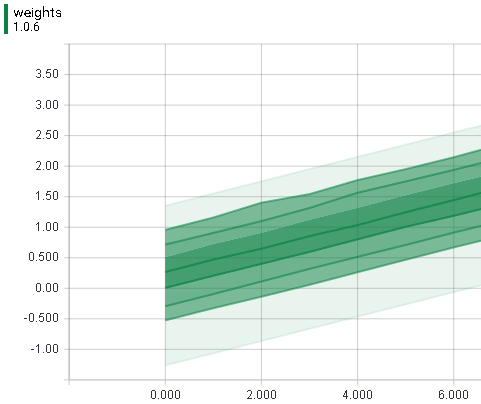
\includegraphics[scale=0.8]{images/Distripution-small.png}
	\caption{Verteilung der Werte in einem Tensor über die Zeit}
	\label{fig:Verteilungsdiagram}
\end{figure}
Im Diagramm \ref{fig:Verteilungsdiagram} wird ein Tensor mit 100 Werten dargestellt. 
Dieser Tensor wurde mit einer Normalverteilung initialisiert, wobei die Standardabweichung bei $0.5$ liegt und der Median zu Beginn bei $0.2$, mit einer geringen Abweichung. 
Die Linien in diesem Diagramm und ihre Einfärbungen präsentieren die Verteilung der Werte im beobachteten Tensor. 
Die Verteilung muss von unten nach oben gelesen werden, dabei ergibt die unterste Linie den Minimalwert, der vorgekommen ist. 
Die nächste Linie besagt, dass sich 7\% der Werte im Bereich zwischen dem geringsten und der zweiten Linie befinden, was inklusiv des geringsten Wertes ist.  
Der nächste Bereich definiert, wie in einer gaußschen Normalverteilung, dass sich bis zum Ende dieses Bereiches 16\% darin befinden. 
Im Gesamten sind dies $9$ Markierungen mit 8 Bereichen, welche zusammen alle Werte im Tensor widerspiegeln. 
Diese Folge an prozentualen Anteilen lauten wie folgend: $min, 7\%, 16\%, 31\%, 50\%, 69\%, 84\%, 93\%, max$. 
Im Diagramm \ref{fig:VerteilungsdiagrammPython} ist diese Verteilung besser ersichtlich, zusätzlich befinden sich in der Abbildung \ref{fig:Ergebnistensor} die Rohdaten der Diagramme. 
\begin{figure}
	\centering
	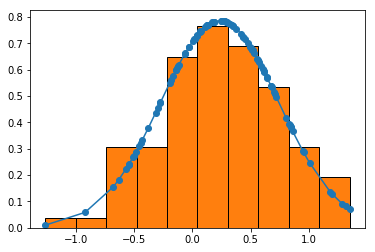
\includegraphics[scale=0.6]{images/gaussian.png}
	\caption{Verteilung der Werte in dem Tensor zu dem Diagramm \ref{fig:Verteilungsdiagram}}
	\label{fig:VerteilungsdiagrammPython}
\end{figure}
\begin{lstlisting}[caption={Sortierter Ergebnistensor zum Verteilungsdiagramm \ref{fig:VerteilungsdiagrammPython} und \ref{fig:Verteilungsdiagram} im Schritt $0$},label=fig:Ergebnistensor,captionpos=b,language=Python]
 -1.2645409,  -0.92252451, -0.68004417,  -0.63273954,  -0.57005012, 
 -0.5477351,  -0.54554129, -0.51146084,  -0.50482351,  -0.4872272, 
 -0.45631331, -0.44180638, -0.43258488,  -0.38066232,  -0.31675094, 
 -0.29567719, -0.27768314, -0.27437925,  -0.19503899,  -0.18343721, 
 -0.16653274, -0.13992153, -0.13946836,  -0.12969615,  -0.12044857, 
 -0.11908005, -0.06734778, -0.062724337, -0.032598898, -0.02885592, 
  0.006216079, 0.015204117, 0.018379062,  0.036883533,  0.041039094, 
  0.063002124, 0.068820029, 0.072805718,  0.11137276,   0.11735194, 
  0.12555882,  0.12613684,  0.13053563,   0.13633718,   0.17283598, 
  0.18271323,  0.18530971,  0.18671049,   0.24375655,   0.25207496, 
  0.27566099,  0.27588493,  0.27921408,   0.28581429,   0.29526407, 
  0.30613232,  0.32309669,  0.33705187,   0.34577289,   0.34687665, 
  0.37553167,  0.41834235,  0.43759531,   0.4376972,    0.45076531, 
  0.47984695,  0.49715465,  0.50634104,   0.51550949,   0.5168677, 
  0.53031796,  0.5579083,   0.56285316,   0.57165861,   0.59320259, 
  0.60513371,  0.61539149,  0.61814398,   0.63975775,   0.64333171, 
  0.67751783,  0.67795348,  0.68242437,   0.70252627,   0.70793462, 
  0.72128826,  0.80693412,  0.83029318,   0.83635086,   0.84400082, 
  0.84558558,  0.86151552,  0.95068389,   0.95598722,   1.0072051, 
  1.1837469,   1.1992682,   1.285683,     1.3168017,    1.3521272
\end{lstlisting}


%[maximum, 93%, 84%, 69%, 50%, 31%, 16%, 7%, minimum]
%[maximum, μ+1.5σ, μ+σ, μ+0.5σ, μ, μ-0.5σ, μ-σ, μ-1.5σ, minimum]

%\textbf{TODO Grafik}

\paragraph{Histogram} passiert auf denselben Daten wie die Verteilungsansicht. 
Im Grunde präsentiert diese Ansicht die Daten nur auf eine andere Art und Weise. 
\begin{figure}
	\centering
	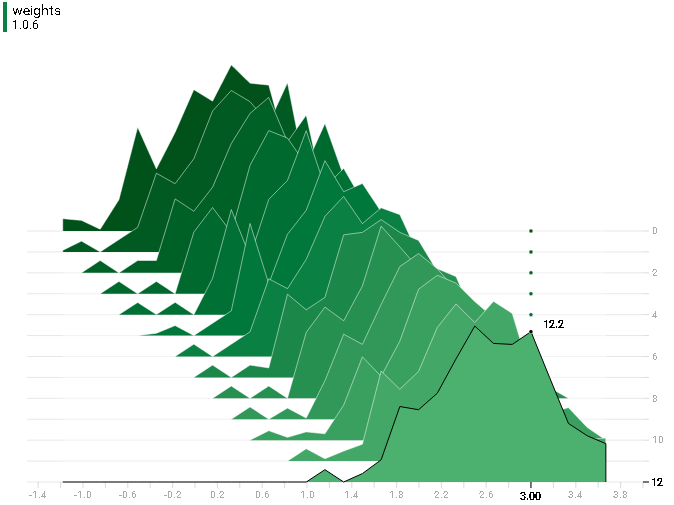
\includegraphics[scale=0.7]{images/histogram-value.png}
	\caption{Verteilung der Werte in dem Tensor in einem Histogramm}
	\label{fig:Histogram}
\end{figure}
Wie auch in der anderen Darstellung werden die Schritte direkt auf einer Achse dargestellt. 
Im Falle des Histogramm \ref{fig:Histogram} ist dies die Achse, welche sich dreidimensional aus dem Hintergrund des Bildes in den Vordergrund zieht. 
Die horizontalen Achsen, welche zu jedem Schritt gezeichnet werden, projizieren ihre Wertebereiche immer auf die vorderste Achse. 
Auf dieser wird der Wertebereich abgebildet, in welchem sich die Werte im Tensor befinden. 
Die Erhebungen und die sich darunter bildenden Flächen geben die Verteilung der Werte wieder. 
So wird beim Überfahren eines Schrittes mit der Maus dieser aktiviert, wie im Histogramm \ref{fig:Histogram} ersichtlich ist. 
Im Falle dieses Diagramms und dieser Stelle bedeutet das, dass sich in der Nähe des Wertes $3.00$ ungefähr $12.2$ Einträge im Tensor befinden. 
Anders ausgedrückt haben $12.2$ konkrete Werte im Tensor den Wert $3.00$ oder einen naheliegenden. 
Durch die Verteilung der Werte entsteht nun der Fall, dass ein Teil der Einträge auch zu einem Wertebereich vorher oder nachher gehören kann. 
Dieses Diagramm stellt die Verteilung in Wertebereiche dar, wobei alle vertikalen Werte in einem Schritt die Anzahl der Werte im Tensor ergeben müssen. 
Im Falle dieses Beispiels ergeben sie aufsummiert einen Wert von $100.044$, was gerundet die $100$ Einträge im Tensor bestätigt. 
Die Aufteilung der Werte in Wertebereiche mit Teilzuweisungen erklärt auch den Schrittverlauf im Histogramm \ref{fig:Histogram}. 
Hier ist ersichtlich, dass sich die Verteilungen und Zugehörigkeiten immer ein wenig vom vorhergehenden abweichen, obwohl in diesem Beispiel in jedem Schritt konstant $0.2$ zu jedem Wert hinzu addiert worden ist. 
Dies lässt sich bei einer geringen Anzahl an Werten, wie hier mit $100$ leichter beobachten, als bei einer sehr viel höheren. \phantom \newline

\noindent
TensorBoard bietet noch weitere Möglichkeiten, wie Bilder- oder Soundinhalte mit in das Event-File zu geben, um diese dann in Tensorboard weiter zu verwenden. 
So können diese Inhalte durch den Graphen gesendet werden und dabei beobachtet werden. 
Die letzte Erweiterung in Tensorboard ist der Punkt mit 'Embedding' \footnote{Online Dokumentation: Emeddings \url{www.tensorflow.org/get_started/embedding_viz}}, wo gelernte Informationen, so wie sie vom Graphen gruppiert worden sind, dargestellt werden können.  \phantom \newline

\noindent
Dieses Kapitel repräsentiert die grundsätzliche Funktionalität des TensorFlow-Systems. 
Dabei wurde auf die Grundlagen und die am meisten benötigten Methoden eingegangen. 
Ihr Verständnis stellt die Grundlage für das nächste Kapitel dar. 
In diesem wird ein praktisches Beispiel mit TensorFlow erläutert. 








